% no answer key
% \documentclass[letterpaper]{exam}

% answer key
\documentclass[letterpaper, landscape]{exam}
\usepackage{2in1, lscape} 
\printanswers

\usepackage{units} 
\usepackage{xfrac} 
\usepackage[fleqn]{amsmath}
\usepackage{float}
\usepackage{mdwlist}
\usepackage{booktabs}
\usepackage{cancel}
\usepackage{polynom}
\usepackage{caption}
\usepackage{fullpage}
\usepackage{comment}
\usepackage{enumerate}
\usepackage{graphicx}
\usepackage{parskip}

\usepackage{mathtools} 

\newcommand{\dg}{\ensuremath{^\circ}} 
\newcommand{\sgn}{\operatorname{sgn}}

\everymath{\displaystyle}
\title{Calculus I \\ Homework Three \\ Section 2.3}
\author{}
\date{\today}

\begin{document}

  \maketitle

  \section{Homework}
    \begin{itemize*}
      \item read Section 2.3
      \item exercises: 1-4, 8-12, 15-30, 35-45, 47, 55, 56
    \end{itemize*}

  I didn't mean to assign 31-34. If I do accidentally assign graphing calculator
  problems in the future, just skip them if you don't have a graphing calculator.

  Sorry about the mistake.

  \ifprintanswers

    \section{Solutions}

    \begin{description}

      \item[1]
        \begin{enumerate}[(a)]
          \item $\lim_{x \to 2} \left[ f(x) + 5g(x) \right] = \boxed{ -6 }$
          \item $\lim_{x \to 2} \left[ g(x) \right]^3 = \boxed{ -8 }$
          \item $\lim_{x \to 2} \sqrt{f(x)} = \boxed{ 2 }$
          \item $\lim_{x \to 2} \frac{3 f(x)}{g(x)} = \boxed{ -6 }$
          \item $\lim_{x \to 2} \frac{g(x)}{h(x)} \boxed{ - \infty }$ 
          \item $\lim_{x \to 2} \frac{g(x) h(x)}{f(x)} \boxed{ 0 }$ 
        \end{enumerate}

      \item[2]
        \begin{enumerate}[(a)]
          \item $\lim_{x \to 2} \left[ f(x) + g(x) \right] = \boxed{ 2 }$
          \item $\lim_{x \to 1} \left[ f(x) + g(x) \right]$ \fbox{ does not exist } 
          \item $\lim_{x \to 0} \left[ f(x) g(x) \right] = \boxed{ 0 } $ 
          \item $\lim_{x \to -1} \left[ \frac{f(x)}{g(x)} \right]$ \fbox{ does not exist }
          \item $\lim_{x \to 2} \left[ x^3 f(x) \right] = \boxed{ 16 } $ 
          \item $\lim_{x \to 1} \sqrt{3 + f(x)} = \boxed{ 2 }$ 
        \end{enumerate}

      \item[3]
        \[
          \lim_{x \to -2} \left( 3x^4 + 2x^2 - x + 1 \right) = \boxed{ 59 }
        \]

      \item[4]
        \[
          \lim_{x \to 2} \left( \frac{2x^2 + 1}{x^2 + 6x - 4} \right) 
              = \boxed{ \frac{3}{4} }
        \]

      \item[8]
        \[
          \lim_{u \to -2} \sqrt{ u^4 + 3u + 6} = \boxed{ 4 }
        \]

      \item[9]
        \[
          \lim_{x \to 4^-} \sqrt{ 16 - x^2 } = \boxed{ 0 }
        \]

      \item[10]
        \begin{enumerate}[(a)]
          \item $f(2)$ is not defined on the left side and is defined on the
            right side

          \item It doesn't matter whether $f(2)$ is defined when determining the
            limit.
        \end{enumerate}

      \item[11]
        \[
          \lim_{x \to 2} \frac{x^2 + x - 6}{x - 2} 
            = \lim_{x \to 2} (x + 3) = \boxed{ 5 } 
        \]

      \item[12]
        \[
          \lim_{x \to -4} \frac{x^2+5 x+4}{x^2+3 x-4} 
            = \lim_{x \to -4} \frac{x+1}{x-1} = \boxed{ \frac{3}{5} } 
        \]

      \item[15]
        \[
          \lim_{t \to -3} \frac{t^2-9}{2 t^2+7 t+3}            
            = \lim_{t \to -3} \frac{t-3}{2 t+1} = \boxed{ \frac{6}{5} } 
        \]

      \item[16]
        \begin{align*}
          \lim_{x \to -1} \frac{x^2-4 x}{x^2-3 x-4} & = \lim_{x \to -1} \frac{x}{x+1}
          \\
          \lim_{x \to -1^-} \frac{x}{x+1}           & = \infty \\
          \lim_{x \to -1^+} \frac{x}{x+1}           & = -\infty \\
        \end{align*}

        Since 
        \[
          \lim_{x \to -1^-} f(x) \neq \lim_{x \to -1^-} f(x)
        \]
        $\lim_{x \to -1} f(x)$ is not defined.

      \item[17]
        \[
          \lim_{x \to 0} \frac{(x+4)^2-16}{x} 
            = \lim_{x \to 0} x + 8 = \boxed{ 8 } 
        \]

      \item[18]
        \[
          \lim_{x \to 1} \frac{x^3-1}{x^2-1} 
            = \lim_{x \to 1} \frac{x^2+x+1}{x+1} = \boxed{ \frac{3}{2} } 
        \]

      \item[19]
        \[
          \lim_{x \to -2} \frac{x+2}{x^3+8} 
            = \lim_{x \to -2} \frac{1}{x^2-2 x+4} = \boxed{ \frac{1}{12} } 
        \]

      \item[20]
        \[
          \lim_{h \to 0} \frac{(h+2)^3-8}{h} 
            = \lim_{h \to 0} h^2+6 h+12 = \boxed{ 12 } 
        \]

      \item[21]
        \[
          \lim_{x \to 9} \frac{9-x}{3-\sqrt{x}} 
            = \lim_{x \to 9} \sqrt{x}+3 = \boxed{ 6 } 
        \]

      \item[22]
        \[
          \lim_{x \to 0} \frac{\sqrt{x+1}-1}{x} 
            = \lim_{x \to 0} \frac{1}{\sqrt{x + 1} + 1} 
            = \boxed{ \frac{1}{2} } 
        \]

      \item[23]
        \[
          \lim_{x \to 7} \frac{\sqrt{x+2}-3}{x-7} 
            = \lim_{x \to 7} \frac{1}{\sqrt{x + 2} + 3} 
            = \boxed{ \frac{1}{6} } 
        \]

      \item[24]
        \[
          \lim_{x \to -1} \frac{x^2+2 x+1}{x^4-1} 
            = \lim_{x \to -1} \frac{x+1}{(x^2+1)(x-1)} 
            = \boxed{ 0 } 
        \]

      \item[25]
        \[
          \lim_{x \to -4} \frac{\sfrac{1}{x}+\sfrac{1}{4}}{x+4} 
            = \lim_{x \to -4} \frac{1}{4 x} 
            = \boxed{ -\frac{1}{16} } 
        \]

      \item[26]
        \[
          \lim_{t \to 0} \frac{1}{t}-\frac{1}{t^2+t} 
            = \lim_{t \to 0} \frac{1}{t + 1} 
            = \boxed{ 1 } 
        \]

      \item[27]
        \[
          \lim_{x \to 16} \frac{4-\sqrt{x}}{16 x-x^2} 
            = \lim_{x \to 16} \frac{1}{x (\sqrt{x} + 4)} 
            = \boxed{ \frac{1}{128} } 
        \]

      \item[28]
        \[
          \lim_{h \to 0} \frac{(h+3)^{-1}-3^{-1}}{h} 
            = \lim_{h \to 0} -\frac{1}{3 h+9} 
            = \boxed{ - \frac{1}{9} } 
        \]

      \item[29]
        \begin{align*}
          \lim_{t \to 0} \frac{1}{t \sqrt{t+1}}-\frac{1}{t} 
            & = \lim_{t \to 0} \frac{1 - \sqrt{1 + t}}{t \sqrt{t+1}} \\
            & = \lim_{t \to 0} \frac{-1}{\sqrt{t+1} (1 + \sqrt{1 + t})} \\
            & = \boxed{ - \frac{1}{2} }
        \end{align*}

      \item[30]
        \begin{align*}
          \lim_{x \to 0} \frac{\sqrt{x^2+9}-5}{x+4} 
            &= \lim_{x \to 0} \frac{x^2+9-25}{\left(x+4\right) \left(\sqrt{x^2+9}+5 \right)} \\
            & = \lim_{x \to 0} \frac{x^2-16}{\left(x+4\right) \left(\sqrt{x^2+9}+5 \right)} \\
            & = \lim_{x \to 0} \frac{x-4}{\sqrt{x^2+9}+5} \\
            & = \boxed{ - \frac{4}{5} }
        \end{align*}

      \item[31]
        \[
          \lim_{x \to 0}  \frac{x}{\sqrt{3 x+1}-1} = \boxed{ \frac{2}{3} }
        \]

        \begin{figure}[H]
          \centering
          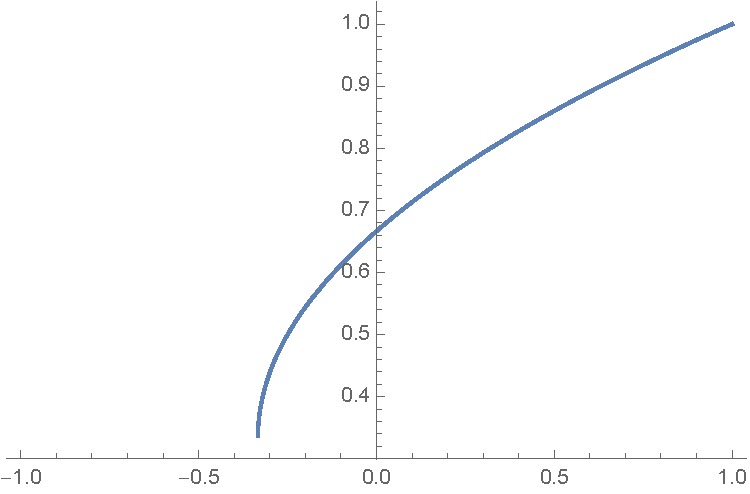
\includegraphics[scale = 0.5]{ex31.pdf}
          \caption{Exercise 31}
          \label{fig:ex31}
        \end{figure}
      \item[32]
        \[
          \lim_{x \to 0} \frac{\sqrt{x+3}-\sqrt{3}}{x} = \boxed{ \frac{1}{2 \sqrt{3}} } 
        \]

        \begin{figure}[H]
          \centering
          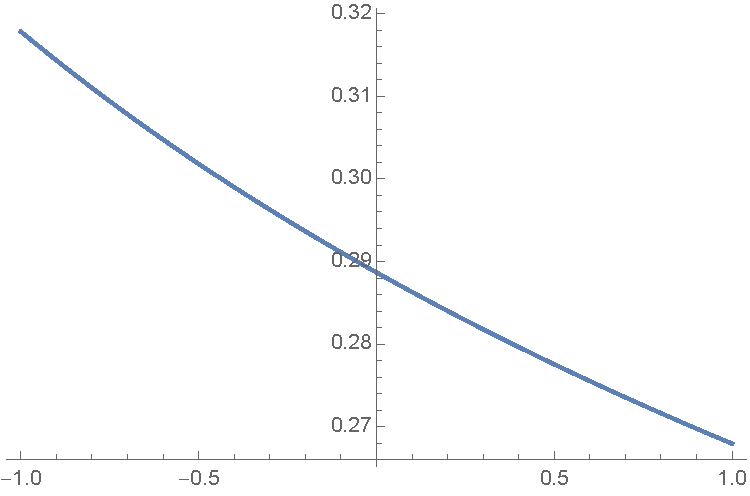
\includegraphics[scale = 0.5]{ex32.pdf}
          \caption{Exercise 32}
          \label{fig:ex32}
        \end{figure}


      \item[33]
        \begin{align*}
          -x^2 \leq x^2 \cos (20 \pi  x) \leq x^2 \\
          \lim_{x \to 0} x^2 \cos (20 \pi  x) = \boxed{ 0 }
        \end{align*}

        \begin{figure}[H]
          \centering
          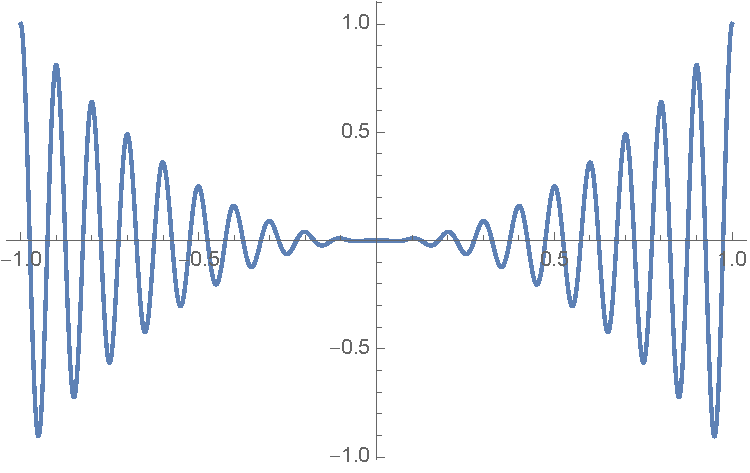
\includegraphics[scale = 0.5]{ex33.pdf}
          \caption{Exercise 33}
          \label{fig:ex33}
        \end{figure}

      \item[34]
        \begin{align*}
          -\sqrt{x^3 + x^2} \leq \sqrt{x^3 + x^2} \sin \left( \frac{\pi}{x} \right) \leq \sqrt{x^3 + x^2} \\
          \lim_{x \to 0} \sqrt{x^3 + x^2} \sin \left( \frac{\pi}{x} \right) = \boxed{ 0 } \\
        \end{align*}

        \begin{figure}[H]
          \centering
          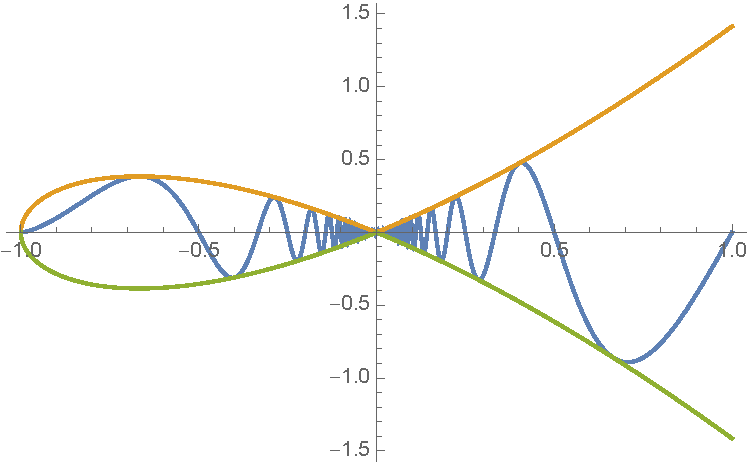
\includegraphics[scale = 0.5]{ex34.pdf}
          \caption{Exercise 34}
          \label{fig:ex34}
        \end{figure}


      \item[35]
        \[
          \lim_{x \to 4} 4x - 9 = \lim_{x \to 4} x^2 - 4x + 7 = 7
        \]

        By the Squeeze Theorem
        \[
          \lim_{x \to 4} f(x) = 7
        \]

      \item[36]
        \[
          \lim_{x \to 1} 2x = \lim_{x \to 1} x^4 - x^2 + 2 = 2
        \]

        By the Squeeze Theorem
        \[
          \lim_{x \to 1} f(x) = 2
        \]

      \item[37]
        The value of the cosine function is always somewhere between $-1$ and
        $1$:
        \[
          -1 \leq \cos \left( \frac{2}{x} \right) \leq 1
        \]

        So:
        \[
          -x^4 \leq x^4 \cos \left( \frac{2}{x}  \right) \leq x^4
        \]

        \[
          \lim_{x \to 0} -x^4 = \lim_{x \to 0} x^4 = 0
        \]

        By the Squeeze Theorem
        \[
          \lim_{x \to 0} x^4 \cos \left( \frac{2}{x} \right) = 0
        \]

      \item[38]
        Since $-1 \leq \sin x \leq 1$,
        \begin{align*}
          e^{-1}      & \leq e^{\sin{\pi/x}} \leq e \\
          \frac{1}{e} & \leq e^{\sin{\pi/x}} \leq e \\
        \end{align*}

        so
        \[
          \frac{\sqrt{x}}{e} \leq e^{\sin \sfrac{\pi}{x}} \sqrt{x} \leq e \sqrt{x}
        \]

        \[
          \lim_{x \to 0+} \frac{\sqrt{x}}{e} = e \sqrt{x} = 0 \\
        \]

        so by the Squeeze Theorem
        \[
          \lim_{x \to 0} e^{\sin \sfrac{\pi}{x}} \sqrt{x} = 0
        \]

      \item[39] 
        \[
          \lim_{x \to 3} (2x + |x - 3|) = \boxed{ 6 } 
        \]

      \item[40]
        \begin{figure}[H]
          \centering
          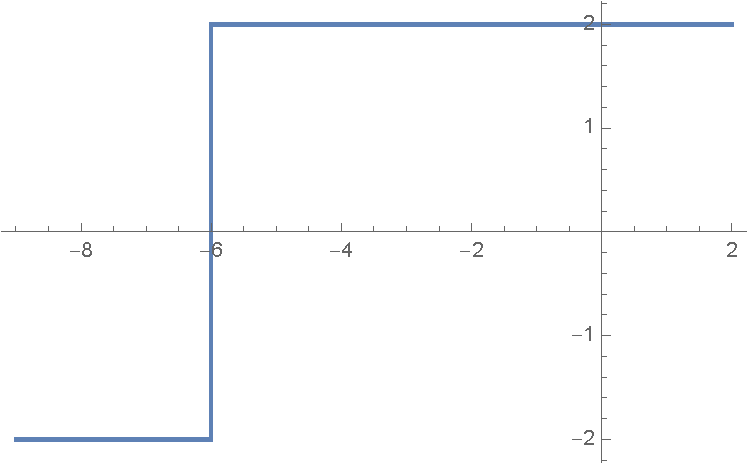
\includegraphics[scale = 0.5]{ex40.pdf}
          \caption{Exercise 40}
          \label{fig:ex40}
        \end{figure}

        \begin{align*}
          \lim_{x \to -6} \frac{2x + 12}{|x + 6|} & = 2 \lim_{x \to -6} \frac{x + 6}{|x + 6|}
          \\
          \lim_{x \to -6^-} \frac{x + 6}{|x + 6|} & = -1 \\
          \lim_{x \to -6^+} \frac{x + 6}{|x + 6|} & = 1 \\
        \end{align*}

        The limit is not defined because 
        \[
          \lim_{x \to -6^-} f(x) \neq \lim_{x \to -6^+} f(x)
        \]

        See Figure \ref{fig:ex40}.

      \newpage

      \item[41]
        \begin{align*}
          f(x) & = \frac{2x - 1}{|2x^3 - x^2|} \\
               & = \frac{1}{x^2} \cdot \frac{2x - 1}{|2x - 1|} \\
        \end{align*}

        \[
          \lim_{x \to -0.5^-} \frac{2x - 1}{x^2 |2x - 1|} = \boxed{ -4 } \\
        \]
        
      \item[42] 
        \[
          \lim_{x \to -2} \frac{2 - |x|}{2 + x} = \lim_{x \to -2} \frac{2 + x}{2 + x} = \boxed{ 1 }
        \]

      \item[43]
        For $x < 0$
        \[
          f(x) = \frac{1}{x} - \frac{1}{-x} = \frac{2}{x}
        \]

        So:
        \[
          \lim_{x \to 0^-} f(x) = \boxed{ - \infty }
        \]

      \item[44]
        For $x > 0$
        \[
          f(x) = \frac{1}{x} - \frac{1}{x} = 0
        \]

        So:
        \[
          \lim_{x \to 0^+} f(x) = \boxed{ 0 }
        \]

      \newpage

      \item[45]
        \begin{figure}[H]
          \centering
          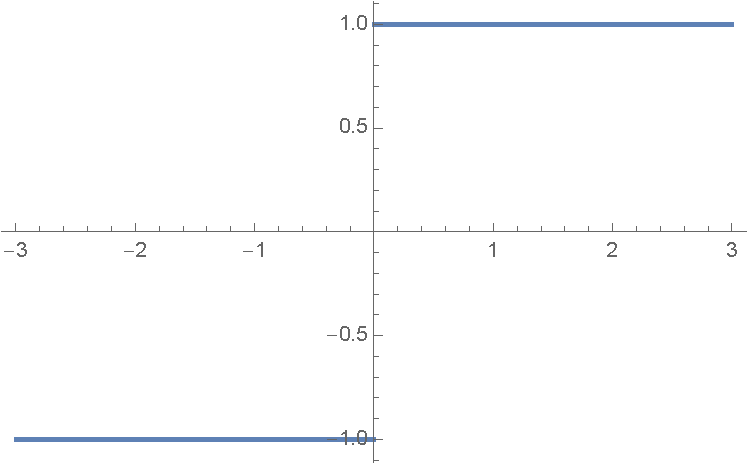
\includegraphics[scale = 0.5]{ex45.pdf}
          \caption{Exercise 45}
          \label{fig:ex45}
        \end{figure}

        \begin{enumerate}[(a)]
          \item see Figure \ref{fig:ex45}
          \item
            \begin{enumerate}[(i)]
              \item $\lim_{x \to 0^+} \sgn x = \boxed{ 1 }$
              \item $\lim_{x \to 0^-} \sgn x = \boxed{ -1 }$
              \item $\lim_{x \to 0} \sgn x$ \fbox{ does not exist }
              \item $\lim_{x \to 0} |\sgn x| = \boxed{ 1 }$
            \end{enumerate}
        \end{enumerate}

      \item[47]
        If $x > 1$: $f(x) = \frac{x^2 - 1}{x - 1} = x + 1$

        If $x < 1$: $f(x) = - \frac{x^2 - 1}{x - 1} = -x - 1$

        \begin{figure}[H]
          \centering
          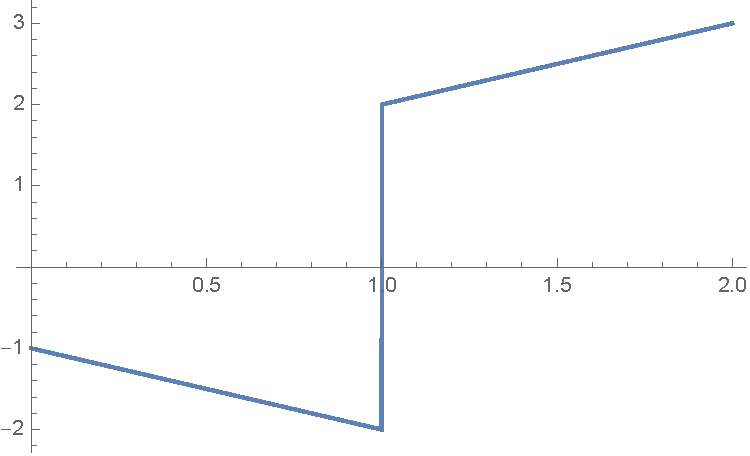
\includegraphics[scale = 0.5]{ex46.pdf}
          \caption{Exercise 46}
          \label{fig:ex46}
        \end{figure}

        \begin{enumerate}[(a)]
          \item
            \begin{enumerate}[(i)]
              \item $\lim_{x \to 1^+} f(x) = \boxed{ 2 }$
              \item $\lim_{x \to 1^-} f(x) = \boxed{ -2 }$
            \end{enumerate}
          \item no, since there are different limits depending on the direction
          \item see Figure \ref{fig:ex46}
        \end{enumerate}

      \item[55]
        \begin{align*}
          \lim_{x \to 1} \frac{f(x) - 8}{x - 1} & = 10 \\
          \lim_{x \to 1} (f(x) - 8)             & = 10 \lim_{x \to 1} (x - 1) \\
          \lim_{x \to 1} (f(x) - 8)             & = 0 \\
          \lim_{x \to 1} f(x)                   & = \boxed{ 8 } \\
        \end{align*}

      \item[56]
        \begin{enumerate}[(a)]
          \item
            \begin{align*}
              \lim_{x \to 0} \frac{f(x)}{x^2} & = 5 \\
              \lim_{x \to 0} f(x)             & = 5 \lim_{x \to 0} x^2 \\
              \lim_{x \to 0} f(x)             & = \boxed{ 0 } \\
            \end{align*}

          \item 
            \begin{align*}
              \lim_{x \to 0} \frac{f(x)}{x^2}                                 & = 5 \\
              \lim_{x \to 0} \frac{f(x)}{x} \cdot \lim_{x \to 0} \frac{1}{x}  & = 5 \\
              \lim_{x \to 0} \frac{f(x)}{x} \cdot  \frac{1}{\lim_{x \to 0} x} & = 5 \\
              \lim_{x \to 0} \frac{f(x)}{x}                                   & = 5 \lim_{x \to 0} x \\
              \lim_{x \to 0} \frac{f(x)}{x}                                   & = \boxed{ 0 } \\
            \end{align*}

        \end{enumerate}
    \end{description}

  \else
    \vspace{11 cm}
    \begin{quote}
      \begin{em}
        Striving for peace and preparing for war are incompatible with each
        other, and in our time more so than ever. 
      \end{em}
    \end{quote}
    \hspace{1 cm} --Albert Einstein
  \fi

\end{document}

